% !TeX root = ../main.tex

\chapter{系统后端设计与实现}
本章节主要介绍系统后端针对不同业务做出的设计,包括数据结构设计和算法设计和实现。

本会议系统的后端涉及到的角色有四种,一是运营人员,二是管理人,三是债权人,四是其他参会人员。涉及到的主要功能有会议基本信息的增删改查、会议的数据导入(包括表决数据导入和其他参会人员信息导入)、直播服务、实时聊天室、实时表决服务等。根据是否和实时性相关将本系统的后端主要分为两个部分,一是非实时服务部分的后端,实现为 SpringBoot 后端; 二是实时服务部分的后端,实现为 WebSocket 后端,后文将对两部分分开进行介绍。

实时服务后端所用到的数据结构全部来自于 SpringBoot 后端,因此数据库设计仅展示 SpringBoot 后端的数据库设计。

\section{数据库设计}
如图~\ref{fig:meetingER}所示,整个系统的数据实体被划分为 Meeting, Schedule,
Group, Ticket, MeetingCreditor, ChatRoom 这 6 种类型的实体以满足需求。其中 Meeting 表示会议, Schedule 表示议程, Group 表示表决组, Ticket 表示选票, ChatRoom 表示会议聊天室。

\begin{figure}[!htp]
    \centering
    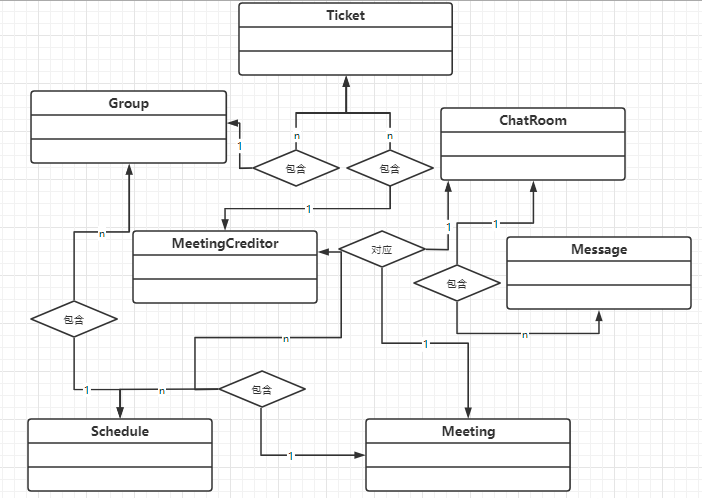
\includegraphics[width=14cm]{meetingER.png}
    \caption{会议系统数据库 ER 图}
    \label{fig:meetingER}
  \end{figure}

本系统使用 Meeting、Schedule、Group 数据实体满足会议信息管理的需求,他们分别表示了会议的基本信息,会议议程信息,议程表决组信息。Meeting 包含了会议的会议名称、创建时间、案件编号以及对应的聊天室 id 等基础信息,Schedule 包含了议程的名称,对应的会议 id ,议程的类型等信息, Group 包含了表决组名称,对应的议程 id 等信息。MeetingCreditor 满足了会议债权人管理的需求,保存着代理人代理的会议债权人的信息。Ticket 满足了投票表决的需求,它包含了选票对应的会议债权人的 id ,对应的表决组 id ,对应的表决金额以及选票的赞成或反对等信息。 ChatRoom 和 Message 满足了实时聊天的需求,其中 Message 包含了所属聊天室 id ,消息内容,发送时间和接收人(接收者的 userId,为空 null 或 [] 则为广播群发)等信息,聊天室包含聊天室的开启状态和禁用用户列表等信息。

\section{非实时后端设计与实现}
非实时后端包含了所有非实时性的功能,主要包括会议基本信息的增删改查、会议的数据导入(包括表决数据导入和其他参会人员信息导入)、其他参会人员登录及直播服务。


\subsection{会议基本信息管理的增删改查}
\subsubsection{创建和修改会议}
在原系统中议程被称为议题,下面统称议程。原系统会议模块创建和修改会议分为三步,分别是填写会议基本信息、填写议程相关信息、导入议程表决信息,只有三步全部完成会议才能创建成功,否则为暂存状态。原本的设计存在一些问题,一是会议创建分为三步过于累赘,导入议程表决信息并不属于创建会议的工作。二是会议和表决强绑定,仅含有无表决议程的会议无法通过导入议程表决信息这一步。

基于以上问题,对创建和修改会议进行了调整。一是将填写会议基本信息和填写议程相关信息合并为一步。在实际实现的时候发现创建会议时,在创建会议请求发送以前,就需要获取会议 id 用于存储会议文件和议程文件至 OSS 文件系统对应会议 id 目录下,因此在创建会议前需要先获取会议 id 。本系统会议的 id 号由 Redis 数据库存储的对应 id 控制,因此在创建会议前,先向 Redis 预约一个会议 id, 在创建会议时将对应会议文件和议程文件存至 OSS文件系统对应目录下,由于从 Redis 中获取 id 后,设置了 id 自增,因此会议 id 号预约唯一。并且由于创建会议时,有多个实体需要存至Mongo数据库,因此实现方法时添加了SpringBoot 的事务性注解,一旦创建会议失败,回滚所有数据库操作。二是将导入议程表决信息从创建修改会议中拆出,仅含有无表决议程的会议也可以正常创建会议,而导入议程表决信息仅有含有需表决议程且导入标记为 false 的会议需要进行,通过这样的设计,仅无表决议程的会议可以正常完成流程。

\subsubsection{删除会议}
原系统会议模块中,删除会议为直接从数据库中删除对应会议全部数据,由于需要规避误删及恶意删除的情况以及需要提供删除恢复的功能,直接从数据库中删除数据的方式不可取,本系统删除操作全部改为采用逻辑删除,对应实体添加 deleted 字段用以表示对应数据是否被删除,为 true 则表示该数据已被删除。

\subsubsection{查询会议}
和原系统会议模块相比,查询会议功能主要有两个重要的变化。一是由于新系统删除操作全部改为逻辑删除,因此在查询时需要根据 deleted 字段进行筛选,获取未被删除的数据。二是原系统会议模块会议的状态是通过获取会议列表事件进行驱动的,在每次获取会议列表时,会对获取到的会议进行一次处理,根据会议召开时间和当前服务器时间的对比重新更新会议状态。在每次获取会议列表时,都会进行这样的操作,假设有 1000 个人拥有1个同样的会议,他们每个人获取一次会议列表,这个会议的状态都会被更新1000遍,即这个会议会被重新存储1000次,如果短时间内大量的人获取会议列表,且每个人会议列表包含的会议数量都不少的情况下,服务器的资源可能很快就被耗尽,这是不可取的。会议的状态仅仅是前端展示的一个维度,不需要存入数据库,只要在获取会议列表时通过会议召开时间和当前服务器时间的对比设置返回给前端的会议状态字段即可。

\subsection{会议系统的数据导入}
会议系统的数据导入分为两个部分,一是表决数据导入,二是其他参会人员信息导入。

原系统的表决数据导入为直接从债权审查模块拉取审查数据,如果用户仅仅使用会议系统而不使用债权审查,会议就无法获取相关数据,会议无法正常进行。这种情况下,会议系统和债权审查系统就变成了强绑定关系,而这是不合理的。因此需要新增额外的导入手段,本系统使用的导入方式是Excel模板导入的方式。用户先从前端点击下载表决数据导入的模板,在填入对应信息后上传表决数据表格,SpringBoot 后端通过逐条读取表决数据表格,导入相关表决信息,若代理人或会议债权人不存在,还需要通过表中信息自动创建代理人和会议债权人,多次导入时,如果对应选票数据存在则进行复用,表中有但数据库中无对应数据的进行创建操作,剩余的上一次导入数据全部逻辑删除,所有存储操作在导入模板数据全部读取完成后进行,若读取发现模板存在错误,则此次导入数据不存回数据库,并将错误信息通过Excel表格返回给用户。表决信息模板如表~\ref{fig:meetingImport}所示。

\begin{table}[h!]
    \begin{center}
      \caption{表决信息导入模板}
      \label{fig:meetingImport}
      \begin{tabular}{c c c c c c }
        \hline
        \textbf{债权人名称} & \textbf{编号} & \textbf{债权所在表决组} & \textbf{表决金额} & \textbf{参会人姓名} & \textbf{参会人手机号} \\
        \hline
        \\
        \hline
      \end{tabular}
    \end{center}
  \end{table}

本系统由于除开参与会议管理的管理人和行使表决权利的债权人外,还有一些其他的参会人员,如法官、无表决权债权人等,只参观会议的进行,不参与其他操作。为了更好地区分,额外设置了其他参会人员,其他参会人员的信息在表决信息导入后,也通过 Excel 表格进行导入,导入方式同表决信息导入,其他参会人员仅参观会议,实际上只在会议进行期间有效,因此其他参会人员信息存入 Redis,无需持久化到 Mongo 数据库,一旦会议结束即可删除。导入其他参会人员信息模板如表~\ref{fig:otherUserImport}所示。

\begin{table}[h!]
    \begin{center}
      \caption{其他参会人员信息导入模板}
      \label{fig:otherUserImport}
      \begin{tabular}{ c c c }
        \hline
       \textbf{参会人姓名} & \textbf{参会人手机号} & \textbf{参会人类型} \\
       \hline
       \\
       \hline
      \end{tabular}
    \end{center}
  \end{table}

在实现了导入后,由于导入模板中存在的新的代理人和会议债权人为系统自动创建,密码也由系统自动创建,而 user 后端的数据加密方式为非对称加密,无法通过数据库中存储的加密 password 字段反向获取明文的密码,因此需要提供自动生成密码的反馈给用户,由于导入可以重复进行,若将密码生成放在导入时,可能会重复进行多次生成密码,这样变相产生浪费。因此改为信息导入都成功后,点击生成密码则会调用生成密码接口自动为对新创建的代理人和会议债权人创建密码,并将生成的密码导出至 Excel 返回并将密码在 OSS文件系统中备份,如果需要再次获取密码,则点击生成密码反馈,直接向 OSS 文件系统请求获取生成密码的 Excel 备份文件。生成密码反馈 Excel 如表~\ref{fig:passwordReturn}所示。

\begin{table}[h!]
    \begin{center}
      \caption{密码反馈模板}
      \label{fig:passwordReturn}
      \begin{tabular}{ c c c c c }
        \hline
       \textbf{用户名称} & \textbf{手机号(登录账号)} & \textbf{密码} & \textbf{用户类型} & \textbf{代理债权人名单} \\
       \hline
       \\
       \hline
      \end{tabular}
    \end{center}
  \end{table}

  \subsection{其他参会人员登录}
  前面提到其他参会人员实际只在会议召开期间有效,且信息不会持久化到 Mongo 数据库,如果使用密码登录,显得比较累赘,因此考虑使用其他登录方式。首先考虑的是使用游客链接登录的方式,直接向其他参会人员发送可以参会的游客链接,点击即可入会参会。管理人反馈使用链接登录和使用账号密码登录对于管理人通知来说是两种参会方式,要减轻管理人的负担,应该让代理人可以通过一致、统一的方式登录,方便管理人沟通,且使用管理人认为链接可以随意转发,会议安全性无法保证。

  游客登录方案不可行,参考目前各系统通用的登录方式后决定使用手机号验证码登录的方式,既可以保证安全性,又不需存储其他参会人员的密码,方便快捷。其他参会人员使用验证码登录时,在 sms 后端生成验证码并通过阿里云短信服务接口向对应手机号发送短信,获得成功反馈后将验证码存至 Redis, 其他参会人员填写发送登录验证请求后,向Redis获取验证码进行对比,若验证码仍在15分钟有效期内,且登录验证码和Redis所存验证码相符合,则登录成功并将 Redis中存储的对应验证码清除。

  \subsection{直播服务}

  \begin{figure}[!htp]
    \centering
    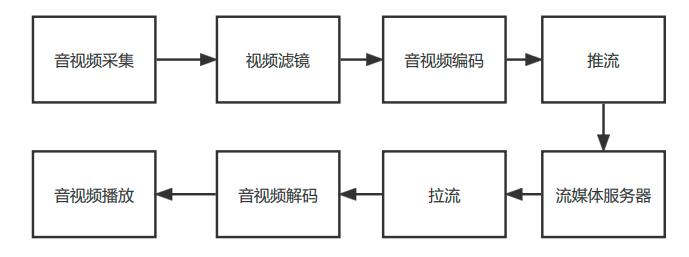
\includegraphics[height=5cm,width=14cm]{live.png}
    \caption{直播服务流程示意图}
    \label{fig:live}
  \end{figure}

  如图~\ref{fig:live}所示,目前直播服务的流程都是先进行音视频采集,然后进行视频的滤镜转换,转换后进行音视频编码,将编码好的音视频推流至流媒体服务器,播放端向流媒体服务器进行拉流,然后对拉取的流进行音视频解码,最后播放。目前本系统直播服务音视频采集、视频滤镜、音视频编码、推流的方式是通过摄像机采集音视频、控制滤镜,音视频编码和推流通过美菲特 M3803 编码器编码并推流。
  流媒体服务器使用的是阿里云直播服务,前端向后端发送请求,后端通过 API 向阿里云直播服务获取拉流地址。

  在使用过程中发现,单一推拉流不够稳定,在长时间的直播中可能出现断线的情况,这对视频表决会议来讲是不可接受的,为了解决这个问题,本系统采取了多路推流的方式,同时将一个直播流向多个推流地址进行推流,当一个推流地址出现问题时,可以通过切换线路保证直播服务的质量。

  \section{实时后端设计与实现}
  实时后端包含了所以具有实时性的服务,包括聊天室服务和实时表决服务。WebSocket后端使用Golang实现。

  \subsection{数据分类}

\begin{figure}[!htp]
  \centering
  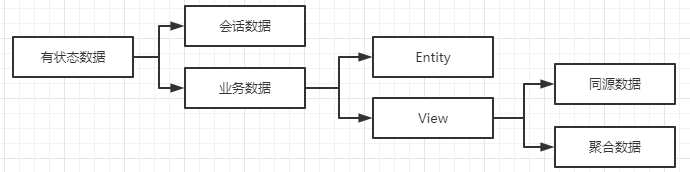
\includegraphics[width=12cm]{dataClassification.png}
  \bicaption[数据分类]
    {数据类型分类示意图}
    {Schematic diagram of data type classification}
 \label{fig:dataClassification}
\end{figure}

如图~\ref{fig:dataClassification},影响实例外在表现的所有副作用数据统称为有状态数据。
有状态数据分为两类,一类是会话数据,一类是业务数据。其中会话数据及业务数据中的Entity数据存于 Redis 中,其余数据均只存于实例内存中。

会话数据为连接的元信息,例如用户 Id ,聊天室 Id , jwt 验证信息等等。
在用户刚刚与实例建立连接时,实例将初始化好用户的会话数据并将其暂存于 Redis 中。
会话数据为每个用户对每个服务的独有数据,包含用户、连接、权限三者的元信息。
用户下线后,会话数据将会被清除。
同用户异地登录,所建立的会话会将原有会话顶替下线(实时服务一账号只可一人用)。

业务数据为影响用户前端展示的数据。例如:某债权人的表决情况,某会议的总签到人数等。
业务数据又分为 View 和 Entity 两种数据。

Entity 为 Mongo 中存储的真实数据,实例会将其暂存于 Redis 中。View 数据是抽象概念,指将对某类用户前端视图展现的全量信息。例如:管理人可见的表决统计总表数据,或者整个聊天室的所有聊天内容和封禁状态。View 并非 Mongo 内的实体数据,往往是多个 Entity 的聚合数据,或者是全体 Entity 的子集。View 数据内部包含同源数据与聚合数据两类。

同源数据是全体 Entity 的子集,内存中为至 Entity 的索引。以保证完全与 Entity 数据保持一致。比如某债权人对某表决是否投票,投了同意还是反对。

聚合数据是由 Entity 聚合而出的数据,会随着某些 Entity 的改变而改变。比如某个会议下某议题的总同意金额。

同源数据和聚合数据采用不同结构存储。它们的区分是调和 “性能” 与 “数据一致性” 矛盾的基石,下节数据存储将会介绍。

\subsection{数据存储}

\begin{figure}[!htp]
  \centering
  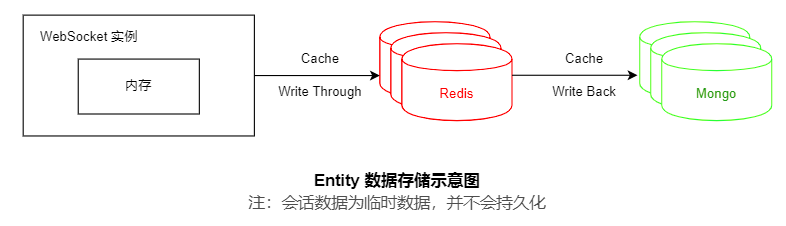
\includegraphics[width=12cm]{dataSave.png}
  \bicaption[Entity存储示意]
    {Entity存储示意图}
    {Entity Storage Diagram}
 \label{fig:dataSave}
\end{figure}

不同类的业务数据存储形式不同。Entity 数据最终会持久化至 Mongo。Entity 被分散到三处。实例内存是 Redis 的 Cache,而 Redis 事实上是 Mongo 的 Cache。

实例必须无状态,其状态必须可从 Redis 恢复。因此实例内存至 Redis 为 Write Through 策略。本⽂的第 5.2.2 节的实验已表明,3 个节点组成的单 Master 的 Mongo 集群仅⽀持 700+ 左右的 QPS,为性能瓶颈。因此 Redis 至 Mongo 为 Write Back 策略。如图~\ref{fig:dataSave}所示。

View 数据只保存在实例内存中。View 内部存储的同源数据事实上只是到某些 Entity 的映射(id、指针等)。View 内部存储的聚合数据是对应的聚合后的计算值。由于 View 内部存储的事实上只是 Entity 的映射,保证 View 的数据一致性的前提下提高了性能。

\subsection{数据推送}

\begin{figure}[!htp]
  \centering
  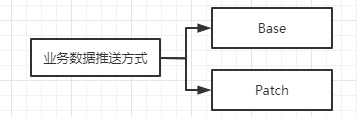
\includegraphics[height=3cm]{dataPush.png}
  \bicaption[推送方式]
    {推送方式示意图}
    {Schematic diagram of push mode}
 \label{fig:dataPush}
\end{figure}

实时系统的核心即后台向前端的数据推送模式。业务数据同时通过 Base 和 Patch 两种方式推送。

Patch 推送则是指对 Entity 与 View 的更新事件。Patch 推送产生的原因可能来自于用户,如某用户发送了一条消息,也可能来自于集群,如结束表决的定时任务到时间了。Patch 推送产生后,先更新 Entity,再更新 View,最后再进行推送。View 数据可通过有序的 Patch 推送计算出来。

Base 推送是指将某个 View 数据推送给前端。Base 推送产生的原因可能来自于用户请求,如初始化内容,也可能来自于服务端的定时推送,如管理人查看表决详情的服务端推送。

\subsection{数据更新}

Entity 数据的更新完全来源于 Patch 推送。

View 数据的更新来源于 Patch 推送以及定时的 Entity 重新聚合计算。Patch 推送可能会更新前端 View 中的 聚合数据。在该策略下,必须进行定时重新聚合计算。定时的重新聚合计算目的是进行 聚合数据 的修正。常规地,在定时重新聚合计算完成后,一个 Base 推送应该被发起。

同源数据并不会被主动更新,因为它是到 Entity 的引用,Entity 被更新则意味着同源数据被更新。

\subsection{数据流}
本节中 “连接” 指 WebSocket 协议的连接,而 “会话” 指用户对服务的请求上下文。
\subsubsection{用户建立会话数据流}
\begin{figure}[!htp]
  \centering
  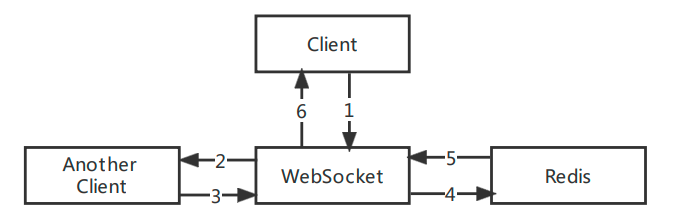
\includegraphics[width=12cm]{createDataflow.png}
  \bicaption[建立数据流]
    {用户建立会话数据流示意图}
    {Schematic diagram of user establishing session data flow}
 \label{fig:createDataflow}
\end{figure}
用户如果要与实例交互,必须先成功建立连接,然后建立会话。
会话是否建立及会话是否存在的判定均以是否建立会话数据,是否存在会话数据为准。
一个用户在同一时刻对一个实时服务只能有一个会话。

1. 客户端向 WebSocket 实例请求搭建连接,实例拿起该用户的会话并且建立锁,然后向 Redis 请求检查用户会话数据:

\quad{}a. 如果已经存在会话数据,并且通过会话数据判定连接未关闭,则转至第 2 步解决异地登陆。

\quad{}b. 如果已经存在会话数据,并且通过会话数据判定连接已关闭,则转至第 4 步覆盖会话;

\quad{}c. 如果检查发现不存在会话数据,则转至第 4 步建立会话;

2. 实例发现异地登录请求,通过 Redis 中的连接,通知占用会话的用户异地登陆的异常;

3. 实例通过清除 Redis 中的对应会话数据关闭与当前占用会话用户的连接,并且转至第 4 步覆盖会话;

4. 实例生成针对该用户的会话数据,与该用户建立连接,并将会话数据存入 Redis;

5. 实例保存会话数据至内存,同时保存当前连接。此时视为会话已经成功建立;

6. 实例放开该用户的会话建立锁,通知用户,会话建立成功,可以接受推送订阅和推送请求。
\subsubsection{用户请求数据流}
\begin{figure}[!htp]
  \centering
  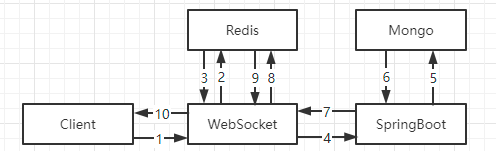
\includegraphics[width=12cm]{requestDateflow.png}
  \bicaption[请求数据流]
    {用户请求数据流示意图}
    {User request data flow diagram}
 \label{fig:requestDateflow}
\end{figure}
框架数据流整体过程如下:

1. 客户端向 WebSocket 实例发送请求:

\quad{}a. 如果 Redis 中已经缓存了相关数据,并且当前请求为读请求,则跳转至第 10 步;

\quad{}b. 如果 Redis 中已经缓存了相关数据,并且当前请求为写请求,则跳转至第 2 步;

\quad{}c. 如果 Redis 中没有相关数据的缓存数据,则直接跳转至第 4 步;

2. 根据写请求的具体要求,WebSocket 实例向 Redis 中写入/更新 Entity 和 View数据;

3. 根据写请求的具体要求,WebSocket 实例将相关数据写入实例内存中,转至第 10 步;

4. 若 Redis 没有缓存数据,则由 WebSocket 实例调用 SpringBoot 后端相关服务接口;

5. SpringBoot 后端向 Mongo 数据库请求获取相关 Entity 数据;

6. Mongo 数据将相关 Entity 数据返回至 SpringBoot 后端中;

7. SpringBoot 后端返回相关 Entity 数据,由 WebSocket 实例计算出相关 View 数据;

8. WebSocket 实例将相关 Entity 数据和 View 数据缓存到 Redis 中;

9. Redis 缓存 Entity 数据和 View 数据成功,WebSocket 也在实例内存中保存对应数据;

10. WebSocket 将请求结果返回给 Client。

  \subsection{WebSocket 业务通信协议}
  在系统的实际业务中,WebSocket 消息传输为双向的。任一端都是 client 和 server。
无论 client 或 server,WebSocket 的所有消息入口只有一个。消息又只发向数个业务中的一个。
并且,根据网络 e2e 通信原则,“at least once” 的请求在业务层必须作出显式响应。
因此,本节将给出所有 WebSocket 业务通信协议的规范和定义,如图~\ref{fig:wsxy}所示。

\begin{figure}[!htp]
    \centering
    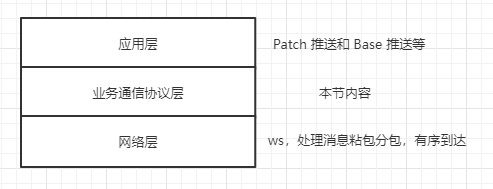
\includegraphics[height=5cm,width=14cm]{wsxy.png}
    \caption{WebSocket 业务通信协议示意图}
    \label{fig:wsxy}
  \end{figure}

  \subsubsection{消息类型}
  Client 与 server 间通信只接受 JSON 格式的 “消息”。
  消息分为多种类型,一种是请求型,一种是相应型,如图~\ref{fig:messageType}所示。
  
  \begin{figure}[!htp]
    \centering
    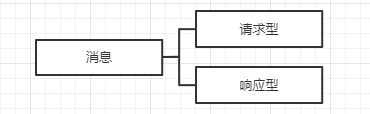
\includegraphics[height=2.5cm]{message.png}
    \caption{消息类型}
    \label{fig:messageType}
  \end{figure}

  请求型消息,可由 client 或 server 发起,向对方请求内容或推送内容,格式如下方代码展示。
  {\setmainfont{Courier New Bold}
\begin{lstlisting}
    // 请求型消息
    {
        "t": "req",    // type
        "i": string,   // 消息 id。为随机数。如果 id 为 0,则代表该请求无需对方响应
        "h": string,   // handler。即 server 对应处理方法名
        "d": object    // data
    }
 \end{lstlisting}}

 响应型消息,对请求型消息的回复,格式如下方代码展示。
 {\setmainfont{Courier New Bold}
 \begin{lstlisting}
    // 响应型消息
    {
        "t": "res",    // type
        "i": string,   // 所响应的请求型消息的 id
        "s": number,   // HTTP 状态码,与 Restful 接口对齐,即可复用 Restful 接口的代码
        "d": object    // data
    }
  \end{lstlisting}}

  \subsubsection{消息处理}
  WebSocket 连接的每一进程都同为 server 和 client,且每一进程的所有消息同享一个入口。
对于每一个 WebSocket 进程:

\quad{}1. 作为 server 时会注册一系列方法,用于处理 d 字段的数据。

\quad{}2. 作为 client 时会发送一系列消息,并等待响应结果返回给上层。

两进程的通信如图~\ref{fig:wsConnect}所示,蓝色 server 和 client 为同一进程,而黄色为另一进程,它们互相通信。
\begin{figure}[!htp]
    \centering
    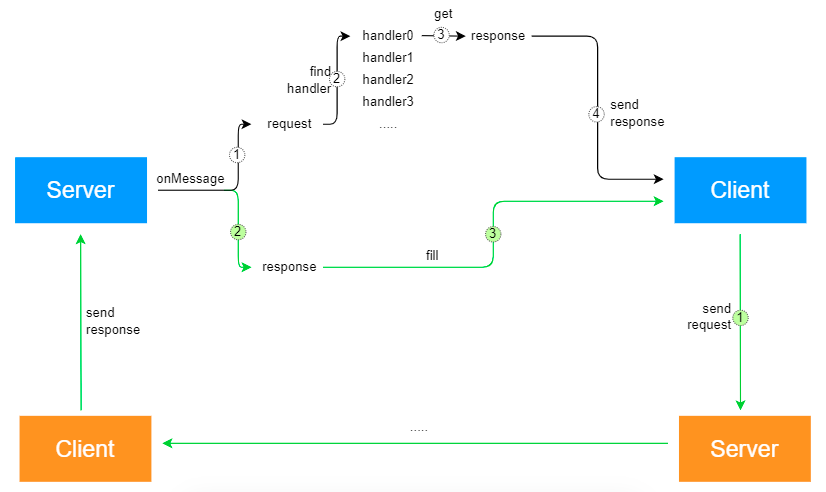
\includegraphics[height=7.5cm]{wsConnect.png}
    \caption{消息处理}
    \label{fig:wsConnect}
  \end{figure}

白色数字标识 server 服务流程:

\quad{}1. 服务端收到信息,检测 t 字段为 req,即为请求;

\quad{}2. 根据信息 h 字段,寻找对应的 handler 以处理 d 字段中的数据;

\quad{}3. Handler 返回请求结果。注意,若未找到 handler,则用默认 handler,返回错误信息;

\quad{}4. 使用本实例的 client,向黄色进程发送返回结果,流程结束;

绿色数字标识 client 需要 server 响应的请求流程:

\quad{}1. client 发送请求消息。上下文进入等待状态。若超时后则 abort(非幂等请求除外);

\quad{}2. 进程执行上文 server 相同流程。流程结束后,本进程收到对应请求的响应消息;

\quad{}3. 将响应消息填充向处于等待状态中的请求上下文,结束等待。

对于不需要 server 响应的 client,其发送的请求中 i 字段为 0。

\subsubsection{Golang 端}
Golang 端中的一份 WebSocket 连接分为两个协程处理,分别进行读操作和写操作的同步。
一个连接所涉及的所有协程均采用 context 进行结束。

Golang 端内部有一个 pendings map,专门用于等待用户的响应型请求。
map 的 key 是请求 id,值是响应型消息的指针的 chan(信道)。

如果要写入请求型消息,对于要用户响应的消息,随机生成一个请求 id,向 pendings map 中注册一个 chan(信道),在该 chan(信道) 上进行等待。
对于不需要用户响应的请求型消息,保持请求 id 为 0,跳过 pendings map 流程,直接写入即可返回。

如果要写入响应型消息,直接写入即可。

对于收到的请求型消息,根据请求型消息的 h 内容,调用程序内不同的 handler。handler 处理后,生成对应的响应型消息,发送给写协程返还给用户。

对于收到的响应型消息,根据其消息 id,找到 pendings map 中正在等待的 chan(信道),向其中写入该消息,让等待消息的协程结束等待。

\subsubsection{JavaScript 端}
JavaScript 端由于浏览器为单线程执行,因此无需关心同步异步的问题。

JavaScript 端内部有两个 map,一个存所有的 handler,一个存所有在等待的 Promise,kv 结构与 Golang 端类似。

如果要写入请求型消息,如果需要返回,则创建一个随机数作为请求 id,再创建一个 Promise 放入等待 map 中,并返回这个 Promise。
如果不需要用户响应的请求型消息,则保持请求 id 为 0,跳过 Promise 放入等待 map 等过程,直接返回即可。

如果要写入响应型消息,直接写入连接即可。

对于收到的请求型消息,根据请求型消息的 h 内容,调用 handler map 中不同的 handler,待其处理后生成对应的响应型消息,直接写入连接中。

对于收到的响应型消息,在等待 map 中找到对应的 Promise,根据消息的 s 进行 resolve 或 reject。

JavaScript 端代码完全用 class 实现,与 React 交互时会产生函数作为状态无法正确更新的问题,后续需换用自定义 hooks 实现。

\subsection{实时聊天室服务}
聊天室服务用于支持表决会议在线聊天,考虑到聊天室支持私聊,因此,每个用户在聊天室中的可见内容不同,即它们的 View 互不相同。
若聊天室同时服务数千人,则服务内部有数千份 View。
如果对每个人进行完整的 Base 推送,根据性能测试结果不能达到预期。

开销来源于重复 marshal,每个用户的 View 中有大量相同数据。
实时聊天室不同于表决服务,每位用户在聊天室中所见的消息是增量的,每份 View 的内容都是增量的,并且每个人的 View 又很可能重叠。这会导致大量计算开销。

\subsubsection{优化设计}
考虑到聊天室数据的本质是一个只读的,持续增长的消息序列并且聊天室并不存在聚合数据,只有同源数据,不需要定时的重新聚合计算任务。
因此,对连接上同一个聊天室的每个用户而言,可以认为所有人共享一个 View,其内部包括所有人发送的所有信息,只不过在 Base 请求时每个人可见的内容不同。

根据这种考虑,聊天室无需存储每个用户的数千个 View,只需存储一个 View,即一个持续增长的数组。
在这个设想下,系统内每条 Message 都有了先后顺序,它们在数组中的索引有序且唯一。
Message 的先后顺序能让聊天室快速构造 Base 推送。
只有用户知晓其接受到了多少 Message,只需定时告知聊天室,即可反推出所缺失的 Message。
用户请求包括两个字段,自己的最新 Message 索引号,以及自己的已知缺失 Message 数组。
聊天室的响应即 Base,包括用户的已知缺失的,以及用户最新至聊天室最新之间的 Message,如图~\ref{fig:wsChatRoom}所示。
\begin{figure}[!htp]
    \centering
    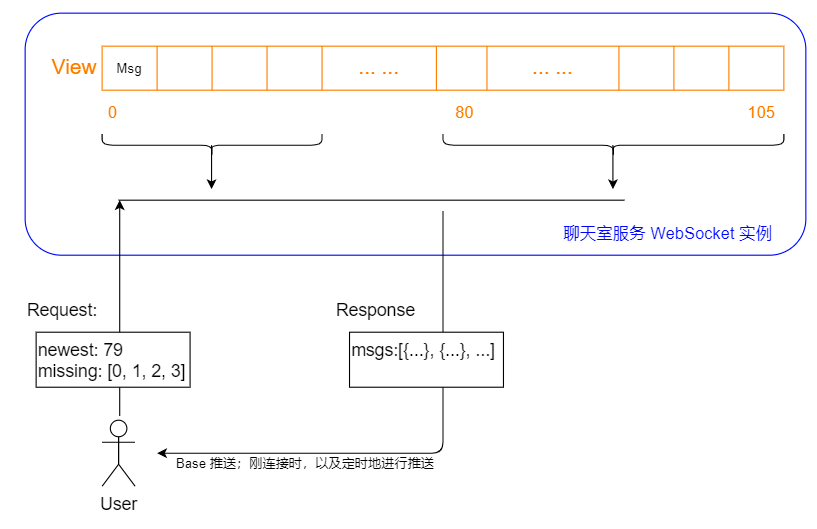
\includegraphics[height=7.5cm]{wsChatRoom.png}
    \caption{聊天室优化方案}
    \label{fig:wsChatRoom}
  \end{figure}

  \subsubsection{重要接口实现}
  本小节展示了聊天室服务一些重要接口的参数和响应,包括会话握手请求,生成 Base 推送,下载聊天记录,发送新消息,封禁和解禁用户,强制用户下线,接受消息推送,接受 ban 推送等。参数和响应若未列出则默认为 null。

  1. Handshake:会话握手请求

  仅限用户发向实例。
  此接口是聊天室服务的基础,用户在使用聊天室服务时,必须在用户握手成功,建立起会话数据后,服务端才会处理用户发来的请求。

  注意,每个用户同一时间不能在多地登陆,如果该用户已经建立了会话数据后,出现异地登录的情况,则强制原先建立的会话下线。

  {\setmainfont{Courier New Bold}
  \begin{lstlisting}
    // 参数:
    {
        "userId": number,
        "chatroomId": number,
        "userType": string, // 用户类型,只接受 PRACTITIONER 和 CREDITOR
        "userName": string
    }
   \end{lstlisting}}

   2. GenerateBase:生成 Base 推送

   仅限用户发向实例。
   实例通过遍历存储消息的 View,返回该用户可见的消息。

   {\setmainfont{Courier New Bold}
   \begin{lstlisting}
    // 参数:
    {
        "missingMsgIds": number[], // 用户已知的缺失的消息 index
        "newestIndex": number // 用户目前收到的最新的消息 index
    }
    // 响应:
    {
        "bannedUsers": number[], // 该用户可见的当前被 ban 的用户 id 列表;管理人可见所有人,债权人只可见自己
        "messages": Message[]
    }
    \end{lstlisting}}

     3. NewMessage:发送新消息

     仅限用户发向实例。
     仅在用户未被 ban 且聊天室未关闭时可用。
     在 View 数组放置一个空消息,放锁,然后将消息存入 Reids。
     操作成功后,该消息会存入 View 数组中对应的空消息处,并引发一次 patch 推送。
  
     {\setmainfont{Courier New Bold}
     \begin{lstlisting}
        // 参数
        Message
        // 响应
        {
            "index": number // 所发送的消息在 View 的消息数组中的 index
        }
      \end{lstlisting}}

      4. Ban:封禁 / 解禁用户

      仅限用户发向实例。此接口仅聊天室未关闭时可用且仅限管理人可用。通过此接口管理员可以对聊天室内的债权人用户进行封禁和解禁操作,此接口不可封禁管理人。

      {\setmainfont{Courier New Bold}
      \begin{lstlisting}
        // 参数
        {
            "userId": number,
            "ban": bool // 指明该用户是否被 ban
        }
       \end{lstlisting}}

       5. ForceOffline:强制用户下线

       仅限实例发向用户。
       聊天室服务不允许同时多地登录,如果用户建立会话时,发现本聊天室已有该用户的会话,则实例会发送给被顶替用户异地登录者的IP和登录时间,并在两秒内关闭原有会话连接。此接口无需响应。

      {\setmainfont{Courier New Bold}
      \begin{lstlisting}
        // 参数
        {
            "time": number, // 异地登录者的登录时间
            "ip": string // 异地登录者的登录 IP
        }
       \end{lstlisting}}

       6. patchMessage:用户接受消息推送

       仅限实例发向用户。
       在用户发送新消息,并成功在消息 View 中保存后,对应的消息会 Patch 推送给发送者和接受者。此接口无需响应。
      {\setmainfont{Courier New Bold}
      \begin{lstlisting}
        // 参数
        Message
       \end{lstlisting}}

  \subsubsection{交互设计}
  考虑到所有用户共享一个 View,其包括所有用户的聊天发言和封禁状态,因此每个用户在前端也维护类似这样的数据结构。具体地,前端维护:

  \quad{}1. messages 数组

  \quad{}2. bannedUsers 数组

对于一个用户来说,其不清楚不可见的信息是由于网络延迟未收到还是由于自己不可见。

对于自己不可见的 message,其 messages 数组对应 index 处为 null,即 JavaScript 语义中的 “有数据但为空”。

对于不确定是不是自己不可见,且又未收到的数据,其 messages 数组对应 index 处为 undefined,即 JavaScript 语义中的 ”不知道“。
对于每个 undefined 的数据,前端会在一定时间内发送 generateBase 请求向后端确认,到底是不是自己不可见,如果不是则返回相应数据。

对于债权人,这样的定时任务为 120s,因为单个债权人看不到其他债权人的发言,因此聊天室内消息不多,服务端向该用户的网络拥塞可能性低。

对于管理人,这样的定时任务为 10s,因为管理人几乎可以看见所有聊天内容,因此聊天室内的消息很多,必须得确保内部的消息的正确性和及时性。

\subsection{实时表决服务}

\subsubsection{实时表决服务流程设计}
以管理人为例,实时表决服务流程如图~\ref{fig:wsbjlc}所示。

\begin{figure}[!htp]
    \centering
    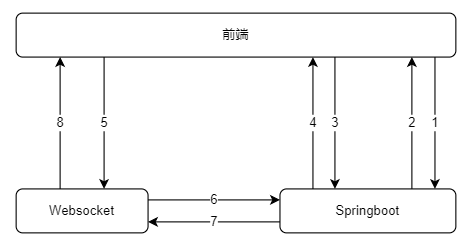
\includegraphics[height=6cm]{wsbjlc.png}
    \caption{WebSocket 表决服务流程示意图}
    \label{fig:wsbjlc}
  \end{figure}

  \quad{}1. 管理人进入会议界面,前端向 SpringBoot 后端发送请求;

  \quad{}2. 后端返回统计数据给前端,前端收到请求后将数据在前端渲染,生成视图,前端接收到数据后需要将数据持久化到客户端上,从而减少后端每次计算全量数据的压力。为了明确前端数据是否需要被更新,后端数据应当给统计数据维护一个类似版本号的字段,若发现版本号变更,则更新数据,重新从 SpringBoot 拉取一遍全量数据;

  \quad{}3. 前端询问会议是否已结束;

  \quad{}4. SpringBoot 返回会议结束标识,若:

  \quad{}\quad{}a. 会议已结束,该流程结束;
  
  \quad{}\quad{}b. 会议未结束,进入第 5 步;
  
  \quad{}5. 会议未结束,则管理人和后端建立 WebSocket 链接,等待数据推送;
  
  \quad{}6. WebSocket 获取会议相关 Entity,数据不存在,向 SpringBoot 发起数据请求,只有 WebSocket 本地没有缓存全量 Entity 时才会向 SpringBoot 返回全量的数据,其他时候直接依据内存 / Redis 返回的缓存计算结果;
  
  \quad{}7. SpringBoot 返回所有的 Entity,WebSocket 将其缓存在 Redis 中,并缓存在内存中;
  
  \quad{}8. WebSocket 根据实际情况实时推送数据到前端,前端依据 WebSocket 推的数据进行更新,WebSocket 不会返回给前端全量的数据,而是一个数据片段,包含各个议题的表决情况、参会人数情况和被更新的数据(比如某自然人就议题 A 提了同意票)。

  \subsubsection{实时表决服务内部数据流和控制流流转}
  WebSocket 会在下列场合和 SpringBoot 的 meeting 服务、前端(债权人端和管理人端)以及 Redis 服务进行通信:

  \quad{}1. 当 WebSocket 的缓存 Redis 没有缓存会议任何数据时,WebSocket 首先要和 SpringBoot 服务通信,获取该会议下全量的 Entity,然后 WebSocket 将这些 Entity 全部存储到 Redis 中,同时在内存中存储一份,它们是一次会议下的 meta 数据;同时,WebSocket 服务会根据得到的 Entity 数据形成一份 View 数据,View 数据表示的是各个议程的统计信息,View 数据不需要持久化到 Redis 中;
  
  \quad{}2. 对于一个债权人而言,假设此时一个债权人投了票,则投票的行为通过前端的 WebSocket 客户端发送到 WebSocket 服务,WebSocket 服务根据收到的投票行为首先更新 Redis 的内存,然后更新对应的内存 Entity 实例,然后将这次表决结果存储在一个 Dirty 中(Dirty 是一段时间内表决 Data 的集合),并更新 View 数据,流程如图~\ref{fig:wszqrlc}所示。

  \begin{figure}[!htp]
      \centering
      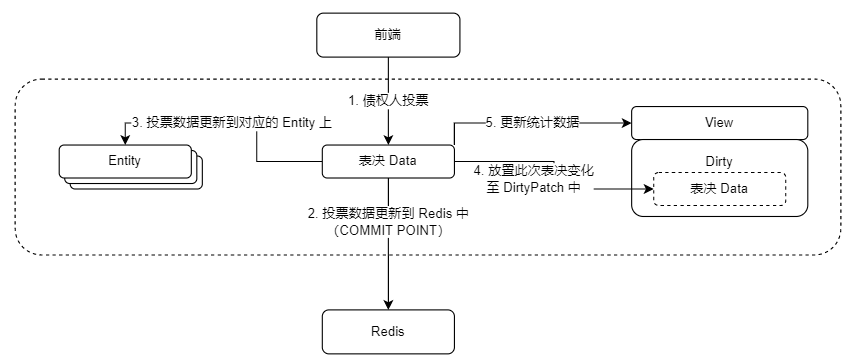
\includegraphics[height=8cm, width=12cm]{wszqrlc.png}
      \caption{债权人投票流程示意图}
      \label{fig:wszqrlc}
    \end{figure}

  \quad{}3. 对于一个管理人而言,其在一开始就已经从 SpringBoot 拿到了所有 Entity,因此只需要接收变化的数据和统计信息:

  \quad{}\quad{}a. 在 WebSocket 链接第一次创建成功时,WebSocket 会向管理人推一次 Base 数据,Base 数据依托于 Entity 数据生成,只记录了投了票/参了会的人员;

  \quad{}\quad{}b. 链接创建成功后,WebSocket 会每隔一段时间(5秒)会检查 Dirty 的数据,如果 Dirty 数据不为空,则向管理人发送 View 和 Dirty 的数据,若中间有数据发送失败,则连接断开。
